
\documentclass[tcc,numbers]{coppe}
% package below turns darkmode on
\usepackage{xcolor} \pagecolor[rgb]{0,0,0} \color[rgb]{1,1,1}
\usepackage{amsmath,amssymb}
\usepackage{silence}
\usepackage{hyperref}

%TODO: remove these two lines when finishing
\setlength{\marginparwidth}{2cm}
\usepackage{todonotes}

\makelosymbols
\makeloabbreviations

\begin{document}
\listoftodos

  \title{Espectro de Modulação Aplicado ao Processamento de Fala}
  % \title{Aplicação do Espectro de Modulação no Processamento de Fala}
  \foreigntitle{Modulation Spectrum Applied over Speech Processing}
  \author{Miguel}{Fernandes de Sousa}
  \advisor{Prof.}{Luiz Wagner}{Pereira Biscainho}{D.Sc.}
  \advisor{Prof.}{Nome do Segundo Orientador}{Sobrenome}{Ph.D.}
  \advisor{Prof.}{Nome do Terceiro Orientador}{Sobrenome}{D.Sc.}

  \examiner{Prof.}{Nome do Primeiro Examinador Sobrenome}{D.Sc.}
  \examiner{Prof.}{Nome do Segundo Examinador Sobrenome}{Ph.D.}
  \examiner{Prof.}{Nome do Terceiro Examinador Sobrenome}{D.Sc.}
  \examiner{Prof.}{Nome do Quarto Examinador Sobrenome}{Ph.D.}
  \examiner{Prof.}{Nome do Quinto Examinador Sobrenome}{Ph.D.}
  \department{ELE}
  \date{07}{2022}

  \keyword{Espectrograma de Modulação}
  \keyword{Filtragem de Modulação}
  \keyword{\textit{Speech Enhancement}}

  %TODO: remover \hbadness
  \hbadness=\maxdimen
  \maketitle

  % \hbadness=\maxdimen
  \frontmatter

  \makecatalog

  \dedication{"Potiusque sero quam nunquam."
  
  Lívio (59 a.C. - 17 d.C.)}
  \hbadness=226

  \chapter*{Agradecimentos}

  Gostaria de agradecer a todos.

  \begin{abstract}

  Apresenta-se, nesta tese, \cite{timit} ...

  \end{abstract}

  \begin{foreignabstract}

  In this work, we present ...

  \end{foreignabstract}

  \tableofcontents
  \listoffigures
  \listoftables
  \printlosymbols
  \printloabbreviations
  \mainmatter
  %%________________________
  %% CHAPTER 01: Introdução
  \chapter{Introdu{\c c}\~ao}
\section{Percepção de periodicidade}
A audição humana é capaz de conferir qualidades subjetivas aos sons, associadas
a parametros físicos nele presentes. Intensidade, timbre, duração e direção percebidas
são exemplos de qualidades subjetivas, enquanto que pressão, frequência,
espectro e envelope são exemplos de parâmetros físicos.\cite{rossing2002}

A audição também é capaz de distinguir sons periódicos de sons "aperiódicos", ou seja,
 sons sem periodicidade definida.

A percepção de periodicidade no sistema auditivo possui qualidades distintas,
 dependendo da frequência do som audível. Frequências abaixo de
20Hz podem ser percebidas ritmicamente, enquanto que frequências audíveis acima de
 20Hz podem ser percebidas como Pitch.

Pitch é a percepção associada à tonalidade do som, na qual o ouvinte é capaz
de distinguir sons agudos e graves, e de ordená-los conforme sua tonalidade.
 Em geral, sons com pitch percebido podem ser representados como a mistura de uma
oscilação no tempo com frequência fundamental, agregada às suas parciais, ou
 harmônicos. Sons ``aperiódicos'' não possuem pitch definido, uma vez que as frequências das
 componentes de sua mistura não são distribuídas harmonicamente. \cite{langner1992} \cite{angus2009} 

 Um som pode ser composto por uma forma de onda periódica, que
 repete-se em função de sua frequência fundamental f, ou período T, sendo essa 
 frequência fundamental percebida como pitch. Essa definição distingue-se de um
 trem de pulsos com determinada taxa de repetição, que não é diretamente
 associada à sua frequência fundamental. Apesar disso, o trem de pulsos pode ser
considerado um som periódico. Os dois casos acima demonstram que o sistema
auditivo realiza tanto uma análise em frequência quanto uma análise no tempo
ao perceber sons. \cite{rossing2002} \symbl{T}{Período} \symbl{f}{Frequência}


A percepção de periodicidade do som também pode ser conferida ao envelope,
definido como a variação no tempo da amplitude ou energia de uma vibração.
Caso o envelope oscile com uma determinada frequência, gera-se uma onda
modulada em amplitude.
Essa modulação pode ser percebida como uma segunda periodicidade,
além da frequência fundamental dessa mesma onda. Dessa forma, vale destacar
que há múltiplas dimensões temporais no estimulo acústico, e pode-se distinguir
a "estrutura fina", associada ao conteúdo espectral, de seu contorno caracterizado
pelo envelope modulado em frequência, ambos compondo a forma de onda no
domínio do tempo. \cite{joris2004}

\citet{langner1992} distingue modulações lentas, abaixo de 20Hz, de
modulações rápidas, entre 20Hz e 1000Hz. Essa distinção se dá pela percepção
distinta nos dois casos: modulações lentas estão associadas à percepção de
ritmo e também à taxa de sequência na construção de palavras, entre 3Hz e 4Hz,
enquanto que modulações rápidas estão associadas a sensação desagradável
de "irregularidade"(roughness) no som. 

\citet{zwicker2013} Apresentam detalhes sobre os limiares de percepção da
Modulação de Amplitude (AM) em função das frequências e intensidades, \citet{joris2004} e
\citet{langner1992} avaliam a resposta à modulação de cada componente do 
sistema auditivo e nervoso, indo além do escopo do
presente trabalho. Modulações temporais são estímulos que auxiliam na detecção,
discriminação, identificação e localização de fontes sonoras,
e esse papel amplo reflete-se em propriedades fisiológicas particulares a cada
componente do sistema auditivo. \abbrev{AM}{Modulação de Amplitude}

Falta falar: brevemente, como o ouvido percebe a modulação ; brevemente, como modulação,
 envelope e formantes da fala se correlacionam; percepção de timbre de instrumentos
  associado ao envelope de cada frequência; inserir imagem.

\section{Descrição do projeto}
\subsection{Objetivos}
\subsection{Organização do Trabalho}
\subsection{Materiais Utilizados}

  %%________________________

  %%________________________
  %% CHAPTER 02
  \chapter{Fundamentação Teórica}
\section{Correspondência entre inteligibilidade e modulação}
% Nervo Auditivo:
% - resolução em frequência e resposta da modulação
% - diversidade de resposta
% - caracteristica passa baixa das fibras do nervo auditivo
% - faixa dinâmica

% Nucleo coclear:
% - resolução em frequência e resposta da modulação
% - diversidade de resposta
% - caracteristica passa baixa das fibras do nervo auditivo
% - faixa dinâmica

% A audição humana pode ser aproximada por um filtro
%  passa-baixas.\cite{langner1992}.

% Modulações abaixo de 20Hz são percebidas ritmicamente. Modulações predominantes
% entre 3 e 4Hz coencidem com a taxa que pronunciamos palavras. \cite{langner1992}.

% Modulações entre 10Hz e 200Hz são percebidas como desagradáveis. \cite{langner1992}.

% \cite{langner1992} define a percepção de periodicidade do envelope como 
% "periodicity pitch". 

% MTF: modulation transfer function.

% A percepção de pitch trata da frequência percebida. Dois sinais complexos
% compostos por diversas componentes frequênciais distintas podem ter o mesmo
%  pitch. Ainda, um sinal, por mais que tenha determinado pitch, pode não conter essa
%  frequência em sua composição. A percepção de pitch funciona por mais que não esteja presente a 
%  frequência fundamental de mesmo valor daquele pitch. \cite{langner1992}

%  Nervo auditivo. Núcleo Coclear. \cite{langner1992}.

%  This indicates that the auditory system tends to separate information about
%   the envelope and the temporal fine structure of a signal as
%    a first step of temporal analysis of sounds.


% Efeito do envelope na percepção de fala:

% \cite{drullman1994} O sinal de fala é caracterizado por um espectro de
%  frequências variante no tempo. Essas variações são responsáveis pela
%  identificação de fonemas, sílabas, palavras e frases.

%  Em todas as bandas, as frequências mais importantes são as presentes entre
%  3 e 4 Hz, refletindo a taxa silábica da fala. É possível encontrar componentes
%  na faixa entre 15-20hz.

%  A sensibilidade para modulação tem caracteristica de um filtro passa-baixa,
%  com queda de 6dB entre 25Hz e 100Hz.

%  Posso colocar um gráfico aqui. Como que se mede esse gráfico?

%  MI: Modulation Index.
%  SRT: Speech-Reception Threshold.
%  STI: Speech-Transmition Index.

%  Em áudio reverberante, a atenuação da modulação diminiu a inteligibilidade de 
%  frases. \cite{drullman1994}. Compressão, por subbandas ou diretamente no sinal,
%  afeta drasticamente a inteligibilidade.

%  Essa informação é útil para síntese de voz? Dado que eu quero sintetizar
%  uma voz com inteligibilidade alta. E para análise do som, em aparelhos para
%  deficientes auditivos?

%  O efeito de borramento é reproduzido em áudio reverberante, ao convoluir
%  um sinal com uma exponencial que decai.

%  Pode ser medida em termos de matriz de confusão.

%  SIQ (sentence intelligibility in quiet).

%  Qual a tradução de smearing? Achatamento, borramento, espalhamento?

%  Detecção de envelope com transformada de Hilbert.
 
% Consoantes são mais afetadas por borramento temporal do que vogais.
\section{Cicloestacionariedade de Segunda Ordem e de Ordem Superior}

\section{Correspondência entre inteligibilidade e modulação}
\section{Speech Enhancement}
˜\newpage 
˜\newpage
\section{STFT}
\newpage 
˜\newpage 
\section{Framework AMS}
\newpage 
˜\newpage 
\section{Espectrograma de modulação}
\newpage 
˜\newpage 
˜\newpage
  %%________________________

   %%________________________
  %% CHAPTER 03
  \chapter{Demodulação}
\section{\textit{Framework} Análise-Modificação-Síntese}
 
O \textit{Framework} análise-modificação-síntese (AMS) é o procedimento que
realiza as etapas de análise com a STFT do sinal, modificação no domínio da
frequência acústica e ressíntese do sinal modificado com a STFT
inversa \cite{paliwal2015}. Caso o sinal de entrada esteja
impregnado por ruído, é possível, de posse de uma estimativa da parcela ruidosa,
subtraí-la do sinal impregnado no domínio da frequência.

Há diferentes métodos e algoritmos para a etapa de modificação no domínio
acústico, os quais também podem ser aplicados no domínio na modulação.
Geralmente, nesse procedimento, a modificação é realizada no módulo do sinal
impregnado no domínio da frequência, preservando a fase.

Assumimos um sinal impregnado por ruído: 
\begin{equation}\label{chap_04:base}
    x[n] = s[n] + d[n]
\end{equation}
em que $s[n]$ e $d[n]$ são as parcelas de sinal e de ruído, respectivamente. No
contexto de \textit{Speech Enhancement}, $s[n]$ é o sinal de fala. O objetivo
final é obter a estimativa $\hat{s}[n]$ mais próxima possível de $s[n]$.

Ao retomar a equação \ref{stft}, temos o sinal impregnado no domínio acústico
em função da STFT das parcelas $s[n]$ e $d[n]$, representadas por $S[l, k]$ e
$D[l, k]$:
\begin{equation} \label{chap_3:stft_sum}
    X[l, k] = S[l, k] + D[l, k],
\end{equation}
cuja representação em fasor é dada por:
\begin{equation}
    X[l, k] = |X[l, k]| e^{j\angle{X[l, k]}}
\end{equation}
em que $|X[l, k]|$ e $e^{j\angle{X[l, k]}}$ são módulo e fase do espectro
acústico. A subtração espectral, um dos métodos de \textit{Speech Enhancement},
estima o espectro da parcela ruidosa $d[n]$ a partir de pausas na fala contidas
em $s[n]$.

O \textit{framework} AMS para \textit{Speech Enhancement} no domínio acústico é
ilustrado no diagrama \ref{se_acoustic}. A etapa de modificação no domínio
acústico retorna $|\hat{S}[l, k]|$, que representa a estimativa do módulo do
sinal desejado. Assume-se que sua fase é igual a de $X[l, k]$. Dessa forma, a
estimativa do sinal desejado no domínio acústico é dada por $|\hat{S}[l,
k]|e^{j\angle{X[l, k]}}$. Ao efetuar a STFT inversa desse sinal, obtém-se a
estimativa $\hat{s}[n]$ do sinal desejado no domínio do tempo. O procedimento é
ilustrado no diagrama \ref{se_acoustic}.

\begin{figure}[h]
    \label{se_acoustic}
    \centering
    \begin{tikzpicture}[auto,>=latex']
        \tikzstyle{block} = [draw, shape=rectangle, minimum height=3em, minimum
        width=3em, node distance=2cm, line width=1pt]
        %Creating Blocks and Connection Nodes
        \node at (0,0) (input) {$x[n]$};
        \node [block, below of=input] (stft) {STFT no domínio acústico};
        \node [below of=stft, node distance=5em] (abs) {$|X[l, k]|$};
        \node [block, below of=abs] (s_e) {\textit{Speech Enhancement no domínio acústico}};
        \node [right of=s_e, node distance=3in] (angle) {$e^j{\angle{X[l, k]}}$};
        \node [block, below of = s_e] (estimativa) {$|\hat{S}[l, k]|e^{j\angle{X[l, k]}}$};
        \node [block, below of=estimativa] (istft) {ISTFT no domínio acústico};
        \node [below of=istft, node distance=5em] (final) {$\hat{s}[n]$};
        
        % \node [left of=sintese, node distance=2.5cm] (output) {$x'[n]$};
        %Connecting Blocks
        \begin{scope}[line width=1pt]
            \draw[->] (input) -- (stft);
            \draw[->] (stft) -- (abs);
            \draw[->] (abs) -- (s_e);
            \draw[->] (s_e) -- (estimativa);
            \draw[->] (stft) -| (angle);
            \draw[->] (angle) |- (estimativa);
            \draw[->] (estimativa) -- (istft);
            \draw[->] (istft) -- (final);
        \end{scope}
    \end{tikzpicture}
    \caption{\textit{Framework AMS para Speech Enhancement no domínio acústico}.}
\end{figure}

Por sua vez, o \textit{framework AMS} para o domínio da modulação é ilustrado no
 diagrama \ref{se_modulation}. Aplica-se a STFT no domínio da modulação ao
 módulo do espectro no domínio acústico, obtendo $|\mathcal{X}[l, k, \mu]|$ e
 $e^{j\angle{\mathcal{X}[l, k, \mu]}}$, que são o módulo e fase do espectro de
 modulação.

\begin{figure}[!ht]
    \label{se_modulation}
    \centering
    \begin{tikzpicture}[auto,>=latex']
        \tikzstyle{block} = [draw, shape=rectangle, minimum height=3em, minimum
        width=3em, node distance=2cm, line width=1pt]
        %Creating Blocks and Connection Nodes
        \node at (0,0) (input) {$x[n]$};
        \node [block, below of=input] (stft) {STFT no domínio acústico};
        \node [below of=stft, node distance=5em] (abs) {$|X[l, k]|$};
        \node [block, below of=abs] (stft_mod) {STFT no domínio da modulação};
        \node [below of=stft_mod, node distance=5em] (abs_mod) {$|\mathcal{X}[l, k, \mu]|$};
        \node [block, below of = abs_mod] (estimativa_mod) {$|\hat{\mathcal{S}}[l, k, \mu]|e^{j\angle{X[l, k]}}$};
        \node [right of=abs_mod, node distance=5cm] (angle_mod) {$e^j{\angle{\mathcal{X}[l, k, \mu]}}$};
        \node [right of=abs_mod, node distance=8cm] (angle) {$e^j{\angle{X[l, k]}}$};
        \node [block, below of=estimativa_mod] (istft_mod) {ISTFT no domínio da modulação};
        \node [block, below of = istft_mod] (estimativa) {$|\hat{S}[l, k]|e^{j\angle{X[l, k]}}$};
        \node [block, below of=estimativa] (istft) {ISTFT no domínio acústico};
        \node [below of=istft, node distance=5em] (final) {$\hat{s}[n]$};

        %Connecting Blocks
        \begin{scope}[line width=1pt]
            \draw[->] (input) -- (stft);
            \draw[->] (stft) -- (abs);
            \draw[->] (abs) -- (stft_mod);
            \draw[->] (stft_mod) -- (abs_mod);
            \draw[->] (abs_mod) -- (estimativa_mod);
            \draw[->] (estimativa_mod) -- (istft_mod);
            \draw[->] (istft_mod) -- (estimativa);
            \draw[->] (stft) -| (angle);
            \draw[->] (stft_mod) -| (angle_mod);
            \draw[->] (angle) |- (estimativa);
            \draw[->] (angle_mod) |- (estimativa_mod);
            \draw[->] (estimativa) -- (istft);
            \draw[->] (istft) -- (final);
        \end{scope}
    \end{tikzpicture}
    \caption{\textit{Framework AMS para Speech Enhancement no domínio acústico}.}
\end{figure}


% Em seguida, o espectro de modulação é obtido, tal como na equação
% \ref{modspec_stft}.

% Os sinais obtidos pela STFT nos domínios acústico e da modulação, das equações
% \ref{stft} e \ref{modspec_stft} possuem representação em módulo e fase:
% \begin{equation}
%     X[l, k] = |X[l, k]| e^{j\angle{X[l, k]}}
% \end{equation}
% \begin{equation}
%     \mathcal{X}[l, k, \mu ] = |\mathcal{X}[l, k, \mu]| e^{j\angle{\mathcal{X}[l, k, \mu]}}
% \end{equation}
% em que $|X[l, k]|$ e $e^{j\angle{X[l, k]}}$ são módulo e fase do espectro
% acústico, $|\mathcal{X}[l, k, \mu]|$ e $e^{j\angle{\mathcal{X}[l, k, \mu]}}$ são
% módulo e fase do espectro de modulação.

% Após a aplicação do método de \textit{Speech Enhancement} no domínio da
% modulação, obtém-se a o módulo da estimativa
% do sinal $s[t]$ original. Ao compor esse módulo com a fase do sinal impregnado,

% $\mathcal{Y}[l, k, m]$,

\section{Justificativa}

Apesar do maior interesse recente em SBRS, há questões no tema que carecem de
 pesquisa. A maioria dos trabalhos associados apresenta uma nova arquitetura ou
 um novo modelo de aprendizado de máquina que supera o estado da arte a partir
 de um \textit{dataset} público, por mais que existam aplicações em que uma
 variedade de modelos de base de comparação superam modelos mais arrojados.

 Algumas das oportunidades de pesquisa em SBRS são \cite{rec_sys_handbook_2022}:
 \begin{inparaenum}[(1)]
     \item a integração com as preferências de longo prazo do usuário, em que
     trabalhos publicados sob a temática \textit{session-aware} são minoria;
     \item a inclusão dos metadados associados aos itens;
     \item a maior variedade de domínios -- por exemplo: notícias, varejo,
     música -- dos problemas representados pelos \textit{datasets}; e
     \item a inclusão do contexto atual do usuário -- região, clima, etc. --
     durante a existência de determinada sessão\end{inparaenum}.
     
Por sua vez, o conteúdo do aplicativo Indaband é publicado pelos
usuários, sendo interesse da plataforma oferecer as ferramentas e soluções para
que os usuários publiquem com qualidade suas sessões.
\vspace{0.2cm}
\begin{figure}[ht]
    \centering
    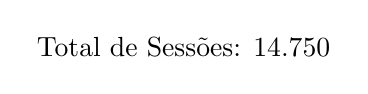
\begin{tikzpicture}
    \pie[ sum=auto, radius=1.4, color={blue!70, orange!70}, after number=\%,
      explode={0, 0.1}, text={}, pos={0,-1}, ]{ 41.3/Publicadas, 58.7/Não
      Publicadas } \node[align=center] at (0,-3) {Total de Sessões: 14.750};
    \end{tikzpicture}
    \hspace{1cm} 
    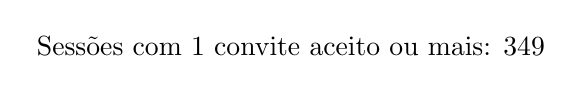
\begin{tikzpicture}
    \pie[ sum=auto, radius=0.8, color={blue!70, orange!70}, after number=\%,
      explode={0, 0.1}, text=legend, pos={0,-1}, ]{ 48.4/Publicadas, 51.6/Não
      Publicadas } \node[align=center] at (0,-3) {Sessões com 1 convite aceito
      ou mais: 349};
    \end{tikzpicture}
    \caption{Sessões e convites enviados. 01/01/2023 a 13/08/2023. Sessões com convites aceitos têm maior taxa de publicação se comparadas ao conjunto completo.}
    \end{figure}
    \vspace{0.2cm}

Sob a perspectiva comercial, o seguinte indício sustenta que um SBRS pode
aumentar a taxa de sessões publicadas pelos usuários do Indaband: apenas 1.146
(7,77\%) das 14.750 sessões criadas em 2023 até 13 de agosto contém no mínimo um
convite emitido. Afunilando ainda mais, a análise das taxas de publicação indica
que as sessões com ao menos um convite aceito, que são apenas 349 (2,37\%) das
14.750 sessões totais criadas, tem maior taxa de publicação se comparada ao
conjunto de todas as sessões. Portanto, uma forma simples de aumentar a taxa de
publicação geral da plataforma é permitir que o conjunto de sessões com
convidados seja maior, o que pode ser incentivado ao integrar um SBRS ao
aplicativo.

Sob a perspectiva de viabilidade técnica, de todas as 14.750 sessões criadas
em 2023 até 13 de agosto, 6.857 (46,5\%) foram criadas com ao menos dois
usuários que gravaram as faixas existentes. Isso é possível a partir da
funcionalidade de \textit{fork}, que permite a cópia de uma sessão publicada
com suas faixas originais. Basta um novo usuário versionar uma sessão com uma
única faixa de outro usuário para que exista associações entre esse novo
usuário e os demais que o segundo usuário já tenha colaborado.

\vspace{0.2cm}
\begin{figure}[H]
      \centering
      \includegraphics[width=1\textwidth]{chapters/chap01/images/plots/users.png}\vfill
      \includegraphics[width=1\textwidth]{chapters/chap01/images/plots/tracks.png}
      \caption{Dados de sessões em 2023 até o presente momento. A quantidade de \textit{tracks}
       e usuários por sessão sustenta a viabilidade técnica de um modelo de
       aprendizado de máquina para a recomendação de convites.}
      \label{fig:combined}
  \end{figure}
\vspace{0.2cm}


  %%________________________

   %%________________________
  %% CHAPTER 04
  \chapter{\textit{Speech Enhancement} aplicado a \textit{Beamformers}}
\section{\textit{Framework} Análise-Modificação-Síntese}
 
O \textit{Framework} análise-modificação-síntese (AMS) é o procedimento que
realiza as etapas de análise com a STFT do sinal, modificação no domínio da
frequência acústica e ressíntese do sinal modificado com a STFT
inversa \cite{paliwal2015}. Caso o sinal de entrada esteja
impregnado por ruído, é possível, de posse de uma estimativa da parcela ruidosa,
subtraí-la do sinal impregnado no domínio da frequência.

Há diferentes métodos e algoritmos para a etapa de modificação no domínio
acústico, os quais também podem ser aplicados no domínio na modulação.
Geralmente, nesse procedimento, a modificação é realizada no módulo do sinal
impregnado no domínio da frequência, preservando a fase.

Assumimos um sinal impregnado por ruído: 
\begin{equation}\label{chap_04:base}
    x[n] = s[n] + d[n]
\end{equation}
em que $s[n]$ e $d[n]$ são as parcelas de sinal e de ruído, respectivamente. No
contexto de \textit{Speech Enhancement}, $s[n]$ é o sinal de fala. O objetivo
final é obter a estimativa $\hat{s}[n]$ mais próxima possível de $s[n]$.

Ao retomar a equação \ref{stft}, temos o sinal impregnado no domínio acústico
em função da STFT das parcelas $s[n]$ e $d[n]$, representadas por $S[l, k]$ e
$D[l, k]$:
\begin{equation} \label{chap_3:stft_sum}
    X[l, k] = S[l, k] + D[l, k],
\end{equation}
cuja representação em fasor é dada por:
\begin{equation}
    X[l, k] = |X[l, k]| e^{j\angle{X[l, k]}}
\end{equation}
em que $|X[l, k]|$ e $e^{j\angle{X[l, k]}}$ são módulo e fase do espectro
acústico. A subtração espectral, um dos métodos de \textit{Speech Enhancement},
estima o espectro da parcela ruidosa $d[n]$ a partir de pausas na fala contidas
em $s[n]$.

O \textit{framework} AMS para \textit{Speech Enhancement} no domínio acústico é
ilustrado no diagrama \ref{se_acoustic}. A etapa de modificação no domínio
acústico retorna $|\hat{S}[l, k]|$, que representa a estimativa do módulo do
sinal desejado. Assume-se que sua fase é igual a de $X[l, k]$. Dessa forma, a
estimativa do sinal desejado no domínio acústico é dada por $|\hat{S}[l,
k]|e^{j\angle{X[l, k]}}$. Ao efetuar a STFT inversa desse sinal, obtém-se a
estimativa $\hat{s}[n]$ do sinal desejado no domínio do tempo. O procedimento é
ilustrado no diagrama \ref{se_acoustic}.

\begin{figure}[h]
    \label{se_acoustic}
    \centering
    \begin{tikzpicture}[auto,>=latex']
        \tikzstyle{block} = [draw, shape=rectangle, minimum height=3em, minimum
        width=3em, node distance=2cm, line width=1pt]
        %Creating Blocks and Connection Nodes
        \node at (0,0) (input) {$x[n]$};
        \node [block, below of=input] (stft) {STFT no domínio acústico};
        \node [below of=stft, node distance=5em] (abs) {$|X[l, k]|$};
        \node [block, below of=abs] (s_e) {\textit{Speech Enhancement no domínio acústico}};
        \node [right of=s_e, node distance=3in] (angle) {$e^j{\angle{X[l, k]}}$};
        \node [block, below of = s_e] (estimativa) {$|\hat{S}[l, k]|e^{j\angle{X[l, k]}}$};
        \node [block, below of=estimativa] (istft) {ISTFT no domínio acústico};
        \node [below of=istft, node distance=5em] (final) {$\hat{s}[n]$};
        
        % \node [left of=sintese, node distance=2.5cm] (output) {$x'[n]$};
        %Connecting Blocks
        \begin{scope}[line width=1pt]
            \draw[->] (input) -- (stft);
            \draw[->] (stft) -- (abs);
            \draw[->] (abs) -- (s_e);
            \draw[->] (s_e) -- (estimativa);
            \draw[->] (stft) -| (angle);
            \draw[->] (angle) |- (estimativa);
            \draw[->] (estimativa) -- (istft);
            \draw[->] (istft) -- (final);
        \end{scope}
    \end{tikzpicture}
    \caption{\textit{Framework AMS para Speech Enhancement no domínio acústico}.}
\end{figure}

Por sua vez, o \textit{framework AMS} para o domínio da modulação é ilustrado no
 diagrama \ref{se_modulation}. Aplica-se a STFT no domínio da modulação ao
 módulo do espectro no domínio acústico, obtendo $|\mathcal{X}[l, k, \mu]|$ e
 $e^{j\angle{\mathcal{X}[l, k, \mu]}}$, que são o módulo e fase do espectro de
 modulação.

\begin{figure}[!ht]
    \label{se_modulation}
    \centering
    \begin{tikzpicture}[auto,>=latex']
        \tikzstyle{block} = [draw, shape=rectangle, minimum height=3em, minimum
        width=3em, node distance=2cm, line width=1pt]
        %Creating Blocks and Connection Nodes
        \node at (0,0) (input) {$x[n]$};
        \node [block, below of=input] (stft) {STFT no domínio acústico};
        \node [below of=stft, node distance=5em] (abs) {$|X[l, k]|$};
        \node [block, below of=abs] (stft_mod) {STFT no domínio da modulação};
        \node [below of=stft_mod, node distance=5em] (abs_mod) {$|\mathcal{X}[l, k, \mu]|$};
        \node [block, below of = abs_mod] (estimativa_mod) {$|\hat{\mathcal{S}}[l, k, \mu]|e^{j\angle{X[l, k]}}$};
        \node [right of=abs_mod, node distance=5cm] (angle_mod) {$e^j{\angle{\mathcal{X}[l, k, \mu]}}$};
        \node [right of=abs_mod, node distance=8cm] (angle) {$e^j{\angle{X[l, k]}}$};
        \node [block, below of=estimativa_mod] (istft_mod) {ISTFT no domínio da modulação};
        \node [block, below of = istft_mod] (estimativa) {$|\hat{S}[l, k]|e^{j\angle{X[l, k]}}$};
        \node [block, below of=estimativa] (istft) {ISTFT no domínio acústico};
        \node [below of=istft, node distance=5em] (final) {$\hat{s}[n]$};

        %Connecting Blocks
        \begin{scope}[line width=1pt]
            \draw[->] (input) -- (stft);
            \draw[->] (stft) -- (abs);
            \draw[->] (abs) -- (stft_mod);
            \draw[->] (stft_mod) -- (abs_mod);
            \draw[->] (abs_mod) -- (estimativa_mod);
            \draw[->] (estimativa_mod) -- (istft_mod);
            \draw[->] (istft_mod) -- (estimativa);
            \draw[->] (stft) -| (angle);
            \draw[->] (stft_mod) -| (angle_mod);
            \draw[->] (angle) |- (estimativa);
            \draw[->] (angle_mod) |- (estimativa_mod);
            \draw[->] (estimativa) -- (istft);
            \draw[->] (istft) -- (final);
        \end{scope}
    \end{tikzpicture}
    \caption{\textit{Framework AMS para Speech Enhancement no domínio acústico}.}
\end{figure}


% Em seguida, o espectro de modulação é obtido, tal como na equação
% \ref{modspec_stft}.

% Os sinais obtidos pela STFT nos domínios acústico e da modulação, das equações
% \ref{stft} e \ref{modspec_stft} possuem representação em módulo e fase:
% \begin{equation}
%     X[l, k] = |X[l, k]| e^{j\angle{X[l, k]}}
% \end{equation}
% \begin{equation}
%     \mathcal{X}[l, k, \mu ] = |\mathcal{X}[l, k, \mu]| e^{j\angle{\mathcal{X}[l, k, \mu]}}
% \end{equation}
% em que $|X[l, k]|$ e $e^{j\angle{X[l, k]}}$ são módulo e fase do espectro
% acústico, $|\mathcal{X}[l, k, \mu]|$ e $e^{j\angle{\mathcal{X}[l, k, \mu]}}$ são
% módulo e fase do espectro de modulação.

% Após a aplicação do método de \textit{Speech Enhancement} no domínio da
% modulação, obtém-se a o módulo da estimativa
% do sinal $s[t]$ original. Ao compor esse módulo com a fase do sinal impregnado,

% $\mathcal{Y}[l, k, m]$,

\section{Justificativa}

Apesar do maior interesse recente em SBRS, há questões no tema que carecem de
 pesquisa. A maioria dos trabalhos associados apresenta uma nova arquitetura ou
 um novo modelo de aprendizado de máquina que supera o estado da arte a partir
 de um \textit{dataset} público, por mais que existam aplicações em que uma
 variedade de modelos de base de comparação superam modelos mais arrojados.

 Algumas das oportunidades de pesquisa em SBRS são \cite{rec_sys_handbook_2022}:
 \begin{inparaenum}[(1)]
     \item a integração com as preferências de longo prazo do usuário, em que
     trabalhos publicados sob a temática \textit{session-aware} são minoria;
     \item a inclusão dos metadados associados aos itens;
     \item a maior variedade de domínios -- por exemplo: notícias, varejo,
     música -- dos problemas representados pelos \textit{datasets}; e
     \item a inclusão do contexto atual do usuário -- região, clima, etc. --
     durante a existência de determinada sessão\end{inparaenum}.
     
Por sua vez, o conteúdo do aplicativo Indaband é publicado pelos
usuários, sendo interesse da plataforma oferecer as ferramentas e soluções para
que os usuários publiquem com qualidade suas sessões.
\vspace{0.2cm}
\begin{figure}[ht]
    \centering
    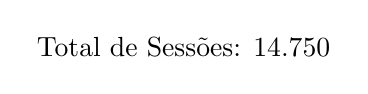
\begin{tikzpicture}
    \pie[ sum=auto, radius=1.4, color={blue!70, orange!70}, after number=\%,
      explode={0, 0.1}, text={}, pos={0,-1}, ]{ 41.3/Publicadas, 58.7/Não
      Publicadas } \node[align=center] at (0,-3) {Total de Sessões: 14.750};
    \end{tikzpicture}
    \hspace{1cm} 
    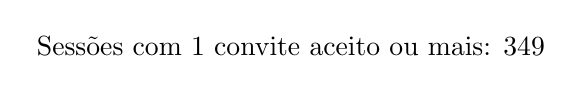
\begin{tikzpicture}
    \pie[ sum=auto, radius=0.8, color={blue!70, orange!70}, after number=\%,
      explode={0, 0.1}, text=legend, pos={0,-1}, ]{ 48.4/Publicadas, 51.6/Não
      Publicadas } \node[align=center] at (0,-3) {Sessões com 1 convite aceito
      ou mais: 349};
    \end{tikzpicture}
    \caption{Sessões e convites enviados. 01/01/2023 a 13/08/2023. Sessões com convites aceitos têm maior taxa de publicação se comparadas ao conjunto completo.}
    \end{figure}
    \vspace{0.2cm}

Sob a perspectiva comercial, o seguinte indício sustenta que um SBRS pode
aumentar a taxa de sessões publicadas pelos usuários do Indaband: apenas 1.146
(7,77\%) das 14.750 sessões criadas em 2023 até 13 de agosto contém no mínimo um
convite emitido. Afunilando ainda mais, a análise das taxas de publicação indica
que as sessões com ao menos um convite aceito, que são apenas 349 (2,37\%) das
14.750 sessões totais criadas, tem maior taxa de publicação se comparada ao
conjunto de todas as sessões. Portanto, uma forma simples de aumentar a taxa de
publicação geral da plataforma é permitir que o conjunto de sessões com
convidados seja maior, o que pode ser incentivado ao integrar um SBRS ao
aplicativo.

Sob a perspectiva de viabilidade técnica, de todas as 14.750 sessões criadas
em 2023 até 13 de agosto, 6.857 (46,5\%) foram criadas com ao menos dois
usuários que gravaram as faixas existentes. Isso é possível a partir da
funcionalidade de \textit{fork}, que permite a cópia de uma sessão publicada
com suas faixas originais. Basta um novo usuário versionar uma sessão com uma
única faixa de outro usuário para que exista associações entre esse novo
usuário e os demais que o segundo usuário já tenha colaborado.

\vspace{0.2cm}
\begin{figure}[H]
      \centering
      \includegraphics[width=1\textwidth]{chapters/chap01/images/plots/users.png}\vfill
      \includegraphics[width=1\textwidth]{chapters/chap01/images/plots/tracks.png}
      \caption{Dados de sessões em 2023 até o presente momento. A quantidade de \textit{tracks}
       e usuários por sessão sustenta a viabilidade técnica de um modelo de
       aprendizado de máquina para a recomendação de convites.}
      \label{fig:combined}
  \end{figure}
\vspace{0.2cm}

\section{\textit{Speech Enhancement} no Domínio da Modulação}
\subsection{Subtração Espectral no Domínio da Modulação}
\subsection{Filtro de Wiener no Domínio da Modulação}
\subsection{Filtro de Wiener no Domínio da Modulação}
\section{Escopo e Objetivos}
\begin{itemize}
    \item Falar que fazemos recomendação de palcos, em breve faremos de Conteúdo
    \item Falar que é específico de convites
    \item \textit{Benchmark} enquanto objetivo
\end{itemize}
\section{Materiais e Organização do Texto}

O trabalho proposto utiliza o \textit{framework} \textit{open-source}
session-rec \cite{sessionrec} escrito em Python, uma vez que contém uma ampla
variedade de modelos SBRS e métricas de avaliação, replicando o padrão de
pesquisas recentes sobre o tema. Os dados utilizados no trabalho foram cedidos
pela empresa Indaband, na condição de anonimização dos usuários tal como ordena
a Lei Geral de Proteção de Dados \cite{lgpd}. Os experimentos foram realizados
em uma máquina virtual com 12 GB de memória RAM, 75 GB de memória de
armazenamento e GPU NVIDIA Tesla T4.

O presente texto é organizado da seguinte forma: o segundo capítulo introduz a
base teórica e aborda os sistemas de recomendação de forma abrangente,
apresentando as abordagens mais tradicionais e que sustentam a intuição de
modelos mais sofisticados. Em seguida, apresenta a definição formal das
recomendações \textit{session-based} e \textit{session-aware}.

O terceiro capítulo apresenta os modelos específicos de recomendação
utilizados no comparativo, descrevendo suas arquiteturas e funcionamento.

O quarto capítulo apresenta os comparativos realizados em abordagens distintas a
partir do conjunto de dados do aplicativo Indaband, incluindo os resultados das métricas
de desempenho assim como uma análise e discussão desses resultados.

O quinto capítulo discute o desempenho dos modelos a partir das métricas
obtidas. Também apresenta a proposta de trabalhos futuros.
  %%________________________

   %%________________________
  %% CHAPTER 05
  \chapter{Conclusōes}
\section{\textit{Framework} Análise-Modificação-Síntese}
 
O \textit{Framework} análise-modificação-síntese (AMS) é o procedimento que
realiza as etapas de análise com a STFT do sinal, modificação no domínio da
frequência acústica e ressíntese do sinal modificado com a STFT
inversa \cite{paliwal2015}. Caso o sinal de entrada esteja
impregnado por ruído, é possível, de posse de uma estimativa da parcela ruidosa,
subtraí-la do sinal impregnado no domínio da frequência.

Há diferentes métodos e algoritmos para a etapa de modificação no domínio
acústico, os quais também podem ser aplicados no domínio na modulação.
Geralmente, nesse procedimento, a modificação é realizada no módulo do sinal
impregnado no domínio da frequência, preservando a fase.

Assumimos um sinal impregnado por ruído: 
\begin{equation}\label{chap_04:base}
    x[n] = s[n] + d[n]
\end{equation}
em que $s[n]$ e $d[n]$ são as parcelas de sinal e de ruído, respectivamente. No
contexto de \textit{Speech Enhancement}, $s[n]$ é o sinal de fala. O objetivo
final é obter a estimativa $\hat{s}[n]$ mais próxima possível de $s[n]$.

Ao retomar a equação \ref{stft}, temos o sinal impregnado no domínio acústico
em função da STFT das parcelas $s[n]$ e $d[n]$, representadas por $S[l, k]$ e
$D[l, k]$:
\begin{equation} \label{chap_3:stft_sum}
    X[l, k] = S[l, k] + D[l, k],
\end{equation}
cuja representação em fasor é dada por:
\begin{equation}
    X[l, k] = |X[l, k]| e^{j\angle{X[l, k]}}
\end{equation}
em que $|X[l, k]|$ e $e^{j\angle{X[l, k]}}$ são módulo e fase do espectro
acústico. A subtração espectral, um dos métodos de \textit{Speech Enhancement},
estima o espectro da parcela ruidosa $d[n]$ a partir de pausas na fala contidas
em $s[n]$.

O \textit{framework} AMS para \textit{Speech Enhancement} no domínio acústico é
ilustrado no diagrama \ref{se_acoustic}. A etapa de modificação no domínio
acústico retorna $|\hat{S}[l, k]|$, que representa a estimativa do módulo do
sinal desejado. Assume-se que sua fase é igual a de $X[l, k]$. Dessa forma, a
estimativa do sinal desejado no domínio acústico é dada por $|\hat{S}[l,
k]|e^{j\angle{X[l, k]}}$. Ao efetuar a STFT inversa desse sinal, obtém-se a
estimativa $\hat{s}[n]$ do sinal desejado no domínio do tempo. O procedimento é
ilustrado no diagrama \ref{se_acoustic}.

\begin{figure}[h]
    \label{se_acoustic}
    \centering
    \begin{tikzpicture}[auto,>=latex']
        \tikzstyle{block} = [draw, shape=rectangle, minimum height=3em, minimum
        width=3em, node distance=2cm, line width=1pt]
        %Creating Blocks and Connection Nodes
        \node at (0,0) (input) {$x[n]$};
        \node [block, below of=input] (stft) {STFT no domínio acústico};
        \node [below of=stft, node distance=5em] (abs) {$|X[l, k]|$};
        \node [block, below of=abs] (s_e) {\textit{Speech Enhancement no domínio acústico}};
        \node [right of=s_e, node distance=3in] (angle) {$e^j{\angle{X[l, k]}}$};
        \node [block, below of = s_e] (estimativa) {$|\hat{S}[l, k]|e^{j\angle{X[l, k]}}$};
        \node [block, below of=estimativa] (istft) {ISTFT no domínio acústico};
        \node [below of=istft, node distance=5em] (final) {$\hat{s}[n]$};
        
        % \node [left of=sintese, node distance=2.5cm] (output) {$x'[n]$};
        %Connecting Blocks
        \begin{scope}[line width=1pt]
            \draw[->] (input) -- (stft);
            \draw[->] (stft) -- (abs);
            \draw[->] (abs) -- (s_e);
            \draw[->] (s_e) -- (estimativa);
            \draw[->] (stft) -| (angle);
            \draw[->] (angle) |- (estimativa);
            \draw[->] (estimativa) -- (istft);
            \draw[->] (istft) -- (final);
        \end{scope}
    \end{tikzpicture}
    \caption{\textit{Framework AMS para Speech Enhancement no domínio acústico}.}
\end{figure}

Por sua vez, o \textit{framework AMS} para o domínio da modulação é ilustrado no
 diagrama \ref{se_modulation}. Aplica-se a STFT no domínio da modulação ao
 módulo do espectro no domínio acústico, obtendo $|\mathcal{X}[l, k, \mu]|$ e
 $e^{j\angle{\mathcal{X}[l, k, \mu]}}$, que são o módulo e fase do espectro de
 modulação.

\begin{figure}[!ht]
    \label{se_modulation}
    \centering
    \begin{tikzpicture}[auto,>=latex']
        \tikzstyle{block} = [draw, shape=rectangle, minimum height=3em, minimum
        width=3em, node distance=2cm, line width=1pt]
        %Creating Blocks and Connection Nodes
        \node at (0,0) (input) {$x[n]$};
        \node [block, below of=input] (stft) {STFT no domínio acústico};
        \node [below of=stft, node distance=5em] (abs) {$|X[l, k]|$};
        \node [block, below of=abs] (stft_mod) {STFT no domínio da modulação};
        \node [below of=stft_mod, node distance=5em] (abs_mod) {$|\mathcal{X}[l, k, \mu]|$};
        \node [block, below of = abs_mod] (estimativa_mod) {$|\hat{\mathcal{S}}[l, k, \mu]|e^{j\angle{X[l, k]}}$};
        \node [right of=abs_mod, node distance=5cm] (angle_mod) {$e^j{\angle{\mathcal{X}[l, k, \mu]}}$};
        \node [right of=abs_mod, node distance=8cm] (angle) {$e^j{\angle{X[l, k]}}$};
        \node [block, below of=estimativa_mod] (istft_mod) {ISTFT no domínio da modulação};
        \node [block, below of = istft_mod] (estimativa) {$|\hat{S}[l, k]|e^{j\angle{X[l, k]}}$};
        \node [block, below of=estimativa] (istft) {ISTFT no domínio acústico};
        \node [below of=istft, node distance=5em] (final) {$\hat{s}[n]$};

        %Connecting Blocks
        \begin{scope}[line width=1pt]
            \draw[->] (input) -- (stft);
            \draw[->] (stft) -- (abs);
            \draw[->] (abs) -- (stft_mod);
            \draw[->] (stft_mod) -- (abs_mod);
            \draw[->] (abs_mod) -- (estimativa_mod);
            \draw[->] (estimativa_mod) -- (istft_mod);
            \draw[->] (istft_mod) -- (estimativa);
            \draw[->] (stft) -| (angle);
            \draw[->] (stft_mod) -| (angle_mod);
            \draw[->] (angle) |- (estimativa);
            \draw[->] (angle_mod) |- (estimativa_mod);
            \draw[->] (estimativa) -- (istft);
            \draw[->] (istft) -- (final);
        \end{scope}
    \end{tikzpicture}
    \caption{\textit{Framework AMS para Speech Enhancement no domínio acústico}.}
\end{figure}


% Em seguida, o espectro de modulação é obtido, tal como na equação
% \ref{modspec_stft}.

% Os sinais obtidos pela STFT nos domínios acústico e da modulação, das equações
% \ref{stft} e \ref{modspec_stft} possuem representação em módulo e fase:
% \begin{equation}
%     X[l, k] = |X[l, k]| e^{j\angle{X[l, k]}}
% \end{equation}
% \begin{equation}
%     \mathcal{X}[l, k, \mu ] = |\mathcal{X}[l, k, \mu]| e^{j\angle{\mathcal{X}[l, k, \mu]}}
% \end{equation}
% em que $|X[l, k]|$ e $e^{j\angle{X[l, k]}}$ são módulo e fase do espectro
% acústico, $|\mathcal{X}[l, k, \mu]|$ e $e^{j\angle{\mathcal{X}[l, k, \mu]}}$ são
% módulo e fase do espectro de modulação.

% Após a aplicação do método de \textit{Speech Enhancement} no domínio da
% modulação, obtém-se a o módulo da estimativa
% do sinal $s[t]$ original. Ao compor esse módulo com a fase do sinal impregnado,

% $\mathcal{Y}[l, k, m]$,

\section{Justificativa}

Apesar do maior interesse recente em SBRS, há questões no tema que carecem de
 pesquisa. A maioria dos trabalhos associados apresenta uma nova arquitetura ou
 um novo modelo de aprendizado de máquina que supera o estado da arte a partir
 de um \textit{dataset} público, por mais que existam aplicações em que uma
 variedade de modelos de base de comparação superam modelos mais arrojados.

 Algumas das oportunidades de pesquisa em SBRS são \cite{rec_sys_handbook_2022}:
 \begin{inparaenum}[(1)]
     \item a integração com as preferências de longo prazo do usuário, em que
     trabalhos publicados sob a temática \textit{session-aware} são minoria;
     \item a inclusão dos metadados associados aos itens;
     \item a maior variedade de domínios -- por exemplo: notícias, varejo,
     música -- dos problemas representados pelos \textit{datasets}; e
     \item a inclusão do contexto atual do usuário -- região, clima, etc. --
     durante a existência de determinada sessão\end{inparaenum}.
     
Por sua vez, o conteúdo do aplicativo Indaband é publicado pelos
usuários, sendo interesse da plataforma oferecer as ferramentas e soluções para
que os usuários publiquem com qualidade suas sessões.
\vspace{0.2cm}
\begin{figure}[ht]
    \centering
    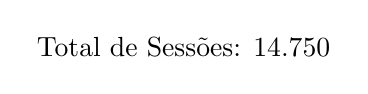
\begin{tikzpicture}
    \pie[ sum=auto, radius=1.4, color={blue!70, orange!70}, after number=\%,
      explode={0, 0.1}, text={}, pos={0,-1}, ]{ 41.3/Publicadas, 58.7/Não
      Publicadas } \node[align=center] at (0,-3) {Total de Sessões: 14.750};
    \end{tikzpicture}
    \hspace{1cm} 
    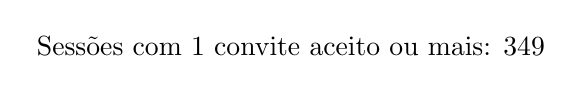
\begin{tikzpicture}
    \pie[ sum=auto, radius=0.8, color={blue!70, orange!70}, after number=\%,
      explode={0, 0.1}, text=legend, pos={0,-1}, ]{ 48.4/Publicadas, 51.6/Não
      Publicadas } \node[align=center] at (0,-3) {Sessões com 1 convite aceito
      ou mais: 349};
    \end{tikzpicture}
    \caption{Sessões e convites enviados. 01/01/2023 a 13/08/2023. Sessões com convites aceitos têm maior taxa de publicação se comparadas ao conjunto completo.}
    \end{figure}
    \vspace{0.2cm}

Sob a perspectiva comercial, o seguinte indício sustenta que um SBRS pode
aumentar a taxa de sessões publicadas pelos usuários do Indaband: apenas 1.146
(7,77\%) das 14.750 sessões criadas em 2023 até 13 de agosto contém no mínimo um
convite emitido. Afunilando ainda mais, a análise das taxas de publicação indica
que as sessões com ao menos um convite aceito, que são apenas 349 (2,37\%) das
14.750 sessões totais criadas, tem maior taxa de publicação se comparada ao
conjunto de todas as sessões. Portanto, uma forma simples de aumentar a taxa de
publicação geral da plataforma é permitir que o conjunto de sessões com
convidados seja maior, o que pode ser incentivado ao integrar um SBRS ao
aplicativo.

Sob a perspectiva de viabilidade técnica, de todas as 14.750 sessões criadas
em 2023 até 13 de agosto, 6.857 (46,5\%) foram criadas com ao menos dois
usuários que gravaram as faixas existentes. Isso é possível a partir da
funcionalidade de \textit{fork}, que permite a cópia de uma sessão publicada
com suas faixas originais. Basta um novo usuário versionar uma sessão com uma
única faixa de outro usuário para que exista associações entre esse novo
usuário e os demais que o segundo usuário já tenha colaborado.

\vspace{0.2cm}
\begin{figure}[H]
      \centering
      \includegraphics[width=1\textwidth]{chapters/chap01/images/plots/users.png}\vfill
      \includegraphics[width=1\textwidth]{chapters/chap01/images/plots/tracks.png}
      \caption{Dados de sessões em 2023 até o presente momento. A quantidade de \textit{tracks}
       e usuários por sessão sustenta a viabilidade técnica de um modelo de
       aprendizado de máquina para a recomendação de convites.}
      \label{fig:combined}
  \end{figure}
\vspace{0.2cm}

  %%________________________

  \backmatter
  
  \bibliographystyle{coppe-unsrt}
  \bibliography{main}

  \appendix
  % \chapter{Algumas Demonstra{\c c}\~oes}
\end{document}
